\documentclass[tikz,border=5pt]{standalone}
\usepackage[UTF8]{ctex}
\usepackage{amsmath,amssymb}
\usetikzlibrary{arrows.meta,calc}
\tikzset{>=Stealth,line cap=round,line join=round,
axis/.style={gray!70,thin,->},aux/.style={gray!55,dashed,thin},
field/.style={blue!65!black,thick},current/.style={red!65!black,thick},
dim/.style={gray!75,<->,thin}}
\newcommand{\outwire}[2]{\draw[fill=white,thick](#1,#2)circle(.09);
\fill(#1,#2)circle(.023);}
\newcommand{\inwire}[2]{\draw[fill=white,thick](#1,#2)circle(.09);
\draw[thick]({#1-.048},{#2-.048})--({#1+.048},{#2+.048});
\draw[thick]({#1-.048},{#2+.048})--({#1+.048},{#2-.048});}
\begin{document}
% 1. Two transverse arrangements. z is normal to each cross-section.
\begin{tikzpicture}[font=\small]
\begin{scope}[x=1.6cm,y=1.6cm]
\draw[axis](-1.65,0)--(1.85,0)node[right,text=black]{$x$};
\draw[axis](0,-1.30)--(0,1.45)node[above,text=black]{$y$};
\inwire{-1}{0}\outwire{1}{0}
\node[above left]at(-1,.09){$-I$};
\node[above right]at(1,.09){$+I$};
\node[below left]at(0,0){$O$};
\draw[aux](-1,0)--(-1,-.75);\draw[aux](1,0)--(1,-.75);
\draw[dim](-1,-.65)--(0,-.65)node[midway,below,text=black]{$\ell$};
\draw[dim](0,-.65)--(1,-.65)node[midway,below,text=black]{$\ell$};
\node at(0,1.90){两导线截面};
\end{scope}
\begin{scope}[xshift=7cm,x=1.6cm,y=1.6cm]
\draw[axis](-1.65,0)--(1.85,0)node[right,text=black]{$x$};
\draw[axis](0,-1.30)--(0,1.45)node[above,text=black]{$y$};
\draw[aux](-1,-1)rectangle(1,1);
\outwire{1}{1}\inwire{-1}{1}\outwire{-1}{-1}\inwire{1}{-1}
\node[above right]at(1,1){$1:\ +I$};
\node[above left]at(-1,1){$2:\ -I$};
\node[below left]at(-1,-1){$3:\ +I$};
\node[below right]at(1,-1){$4:\ -I$};
\node[below left]at(0,0){$O$};
\node[below]at(1,0){$\ell$};
\node[below]at(-1,0){$-\ell$};
\node[right]at(0,1){$\ell$};
\node[right]at(0,-1){$-\ell$};
\node at(0,1.90){四导线截面};
\end{scope}
\node at(3.5,-2.60){$\odot:\ +z,\qquad \otimes:\ -z$};
\end{tikzpicture}
% 2. Parallel wires with a genuine oblique xy plane, not a planar circuit.
\begin{tikzpicture}[font=\small,x={(1.50cm,-.48cm)},
y={(.825cm,.78cm)},z={(0cm,1.35cm)}]
\foreach \a/\b in {1/1,-1/1,-1/-1,1/-1}{
\draw[gray!60,dashed,thick](\a,\b,-1.25)--(\a,\b,0);
\draw[gray!60,densely dotted](\a,\b,-1.65)--(\a,\b,-1.25);
}
\filldraw[fill=blue!6,draw=gray!55](-1.42,-1.42,0)--(1.42,-1.42,0)--
(1.42,1.42,0)--(-1.42,1.42,0)--cycle;
\draw[axis](-1.48,0,0)--(1.85,0,0)node[right,text=black]{$x$};
\draw[axis](0,-1.48,0)--(0,1.85,0)node[above,text=black]{$y$};
\draw[axis](0,0,0)--(0,0,1.85)node[above,text=black]{$z$};
\foreach \a/\b/\n in {1/1/1,-1/1/2,-1/-1/3,1/-1/4}{
\draw[black,thick](\a,\b,0)--(\a,\b,1.25);
\draw[gray!60,densely dotted](\a,\b,1.25)--(\a,\b,1.65);
\fill(\a,\b,0)circle(1.6pt);
\node[below right,inner sep=2pt]at(\a,\b,0){$\n$};
}
\foreach \a/\b in {1/1,-1/-1}{
\draw[current,->](\a,\b,.30)--(\a,\b,.95);
}
\foreach \a/\b in {-1/1,1/-1}{
\draw[current,->](\a,\b,.95)--(\a,\b,.30);
}
\node[below left]at(0,0,0){$O$};
\node[above left]at(-1.42,1.42,0){$xy$ 截面};
\end{tikzpicture}
% 3. Geometry and local signed-vector addition use P=(.2,.6) ell.
\begin{tikzpicture}[font=\small]
\begin{scope}[x=2.1cm,y=2.1cm]
\draw[axis](-1.45,0)--(1.55,0)node[right,text=black]{$x$};
\draw[axis](0,-.20)--(0,1.25)node[above,text=black]{$y$};
\coordinate(P)at(.2,.6);
\inwire{-1}{0}\outwire{1}{0}
\draw[aux](-1,0)--(P)node[midway,above left,text=black]{$r_-$};
\draw[aux](1,0)--(P)node[midway,above right,text=black]{$r_+$};
\fill(P)circle(1.6pt);\node[above]at(P){$P(x,y)$};
\node[below]at(-1,-.08){$(-\ell,0)$};
\node[below]at(1,-.08){$(\ell,0)$};
\node[below left]at(0,0){$O$};
\draw[field,->](P)--(-.10,.20)node[left,inner sep=2pt]{$\boldsymbol B_+$};
\draw[green!40!black,thick,->](P)--(.366667,.266667)
node[right,inner sep=2pt]{$\boldsymbol B_-$};
\end{scope}
\begin{scope}[xshift=7.3cm,yshift=1.5cm,x=2.7cm,y=2.7cm]
\coordinate(S)at(0,0);\coordinate(A)at(-.30,-.40);
\coordinate(T)at(-.133333,-.733333);
\draw[field,->](S)--(A);
\draw[green!40!black,thick,->](A)--(T);
\draw[red!65!black,very thick,->](S)--(T);
\node[above]at(S){$P$};
\node[left]at(-.16,-.17){$\boldsymbol B_+$};
\node[below left]at(-.22,-.57){$\boldsymbol B_-$};
\node[right]at(-.055,-.44){$\boldsymbol B$};
\node at(-.03,.40){首尾相接};
\end{scope}
\end{tikzpicture}
% 4. Exact circle family: neither wire lies on any finite circle.
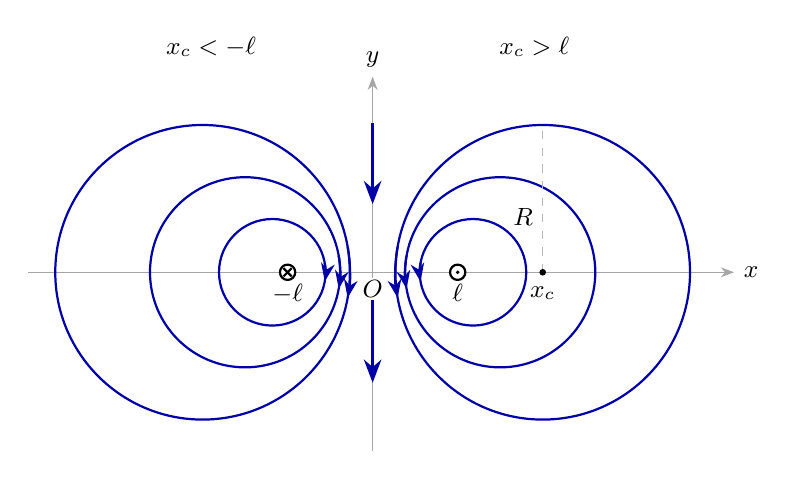
\begin{tikzpicture}[x=1.08cm,y=1.08cm,font=\small]
\draw[axis](-4.05,0)--(4.25,0)node[right,text=black]{$x$};
\draw[axis](0,-2.1)--(0,2.3)node[above,text=black]{$y$};
\foreach \c in {1.18,1.50,2.00}{
\pgfmathsetmacro{\rad}{sqrt(\c*\c-1)}
\draw[field](\c,0)circle(\rad);
\draw[field](-\c,0)circle(\rad);
\draw[field,->]({\c+\rad*cos(170)},{\rad*sin(170)})arc(170:190:\rad);
\draw[field,->]({-\c+\rad*cos(10)},{\rad*sin(10)})arc(10:-10:\rad);
}
\draw[field,very thick,->](0,1.75)--(0,.80);
\draw[field,very thick,->](0,-.30)--(0,-1.30);
\inwire{-1}{0}\outwire{1}{0}
\node[below,yshift=-3pt,fill=white,inner sep=1pt]at(-1,0){$-\ell$};
\node[below,yshift=-3pt,fill=white,inner sep=1pt]at(1,0){$\ell$};
\node[below,fill=white,inner sep=1pt]at(0,-.06){$O$};
\draw[aux](2,0)--(2,1.732051);
\fill(2,0)circle(1.2pt);\node[below]at(2,-.05){$x_c$};
\node[left]at(2,.65){$R$};
\node at(-1.90,2.65){$x_c<-\ell$};
\node at(1.90,2.65){$x_c>\ell$};
\end{tikzpicture}
% 5. Only a small near-origin window is drawn. Axes end at the null.
\begin{tikzpicture}[x=3.8cm,y=3.8cm,font=\small]
\fill[blue!3](-.82,-.82)rectangle(.82,.82);
\draw[aux](-.82,-.82)rectangle(.82,.82);
\draw[axis](-.94,0)--(1.04,0)node[right,text=black]{$x$};
\draw[axis](0,-.94)--(0,1.04)node[above,text=black]{$y$};
\foreach \c in {.10,.22}{
\pgfmathsetmacro{\lo}{\c/.80}
\foreach \signx/\signy in {1/1,1/-1,-1/1,-1/-1}{
\draw[field,domain=\lo:.80,samples=90,smooth,variable=\t]
plot({\signx*\t},{\signy*\c/\t});
\pgfmathsetmacro{\xa}{sqrt(\c)*.94}
\pgfmathsetmacro{\xb}{sqrt(\c)*1.09}
\draw[field,->,domain=\xa:\xb,samples=12,smooth,variable=\t]
plot({\signx*\t},{\signy*\c/\t});
}
}
\draw[field,->](.12,0)--(.65,0);
\draw[field,->](-.12,0)--(-.65,0);
\draw[field,->](0,.65)--(0,.12);
\draw[field,->](0,-.65)--(0,-.12);
\draw[fill=white,thick](0,0)circle(.025);
\node[below right,fill=white,inner sep=1pt]at(0,0){$O$};
\node at(0,1.28){$\boldsymbol B\simeq q(x,-y),\quad q>0$};
\node at(0,-1.18){局部窗口：$|x|,|y|\ll\ell$};
\end{tikzpicture}
\end{document}
